\documentclass[12pt,a4paper]{article}
% \usepackage[condensed,math]{kurier}
% \usepackage[T1]{fontenc}
\usepackage{svg}
\usepackage{tikz}
\usepackage{stanli}
\usepackage{afterpage}
\usepackage{multirow}
\usepackage{subfig}
\usepackage{pgfpages}
\usepackage{svg}
\usepackage{rotating}

\usepackage[lastexercise,answerdelayed]{exercise}
\renewcounter{Exercise}[subsection]
\counterwithin{Exercise}{subsection}
\renewcommand{\ExerciseName}{Esercizio}

\usepackage{listings}
\usepackage{color}

\definecolor{dkgreen}{rgb}{0,0.6,0}
\definecolor{gray}{rgb}{0.5,0.5,0.5}
\definecolor{mauve}{rgb}{0.58,0,0.82}

\lstset{frame=tb,
  language=Java,
  aboveskip=3mm,
  belowskip=3mm,
  showstringspaces=false,
  columns=flexible,
  basicstyle={\small\ttfamily},
  numbers=none,
  numberstyle=\tiny\color{gray},
  keywordstyle=\color{blue},
  commentstyle=\color{dkgreen},
  stringstyle=\color{mauve},
  breaklines=true,
  breakatwhitespace=true,
  tabsize=4
}

% Language setting
% Replace `english' with e.g. `spanish' to change the document language
\usepackage[italian]{babel}

% Set page size and margins
% Replace `letterpaper' with `a4paper' for UK/EU standard size
\usepackage[a4paper,top=2cm,bottom=1.5cm,left=1.5cm,right=1.5cm,marginparwidth=1.75cm]{geometry}

% Useful packages
\usepackage{amsmath}
\usepackage{graphicx}
\usepackage[colorlinks=true, allcolors=blue]{hyperref}

\graphicspath{./images}


\title{}
\author{}
\date{}

\begin{document}
	
	\newcommand{\subf}[2]{%
		{\small\begin{tabular}[t]{@{}c@{}}
				#1\\#2
		\end{tabular}}%
	}
	
	\begin{titlepage}
		\begin{center}
			\vspace*{3cm}
			
			\Huge
			\textbf{Esercizi di Ingegneria del software}
			
			\vspace{0.3cm}
			\Huge
			2023/2024
			
			\vspace{0.8cm}
			\large
			
			%INSTRUCTED BY: MRS. A.A.S.KAUSHLYA
			
			
			\vspace{0.5cm}
			\LARGE
			
			
			\vspace{1.5cm}
			
			\textbf{}
            
\includegraphics[width=0.4\textwidth]{images/uniprLogo.jpg}
			
			\vfill
			
			
			
			\vspace{0.8cm}
			
			
			
			\Large
			
			
			
			
		\end{center}
		\Large
		\begin{tabbing}
			\hspace*{1em}\= \hspace*{8em} \= \kill % set the tabbings
			\> Autori:	\> \textbf{Di Agostino Manuel}, \\
			\>			\>\textbf{Colli Simone}, \\
			\>      	\>\textbf{Merenda Saverio Mattia} \\
			\> Insegnamento:\>  Ingegneria del Software  \\
			\> Anno:  \> 2023/2024
		\end{tabbing}
		
	\end{titlepage}

\tableofcontents
\clearpage
	
\section{Design patterns}
    \subsection{Composite pattern}
    
    \begin{Exercise}\label{composite:ex1}
        Si vuole modellare la mappa di un videogioco \textit{open-world} utilizzando una struttura dati ad albero; a seconda del livello di zoom dell'interfaccia è infatti possibile osservare una versione più dettagliata della mappa, corrispondente ad un particolare nodo dell'albero.
        Esistono quattro categorie di nodi:
        \begin{itemize}
            \item \textbf{foglia}: non ulteriormente espandibile, corrisponde ad un preciso punto fisso sulla mappa, importante per la logica del gioco;
            \item \textbf{distretto}: identifica zone più ampie, ad esempio un quartiere cittadino formato dalla composizione di nodi foglie;
            \item \textbf{regione}: aggrega più distretti contigui;
            \item \textbf{stato}: il livello più alto nella gerarchia considerata.
        \end{itemize}
        Ad ogni nodo sono inoltre sempre associati un \textit{nome} e una \textit{tipologia} conforme alla seguente interfaccia:
        \begin{lstlisting}
    public enum NodeType {
        LEAF,
        DISTRICT,
        REGION,
        COUNTRY
    }
        \end{lstlisting}
        
        Realizzare un class diagram UML che descriva la struttura della soluzione e fornire un'implementazione in Java che ne soddisfi i requisiti.
    \end{Exercise}
    
    \begin{Exercise}\label{composite:ex2} 
    Si vuole realizzare un \textbf{FileSystem} composto da:
        \begin{itemize}
            \item \textbf{Cartelle}: aggregano file o altre cartelle;
            \item \textbf{File}: corrisponde ad un contenuto preciso del FileSystem.
        \end{itemize}
		Realizzare un class diagram UML che descriva la struttura della soluzione e 
		fornirne un'implementazione in Java.
    \end{Exercise}
    %% END COMPOSITE SECTION
    
    
    
    \subsection{Iterator pattern}
    \begin{Exercise}
    \small\textbf{[Richiede \hyperlink{composite:ex1}{\ref{composite:ex1}}]} \\
        È necessario implementare una serie di attraversamenti della struttura dati descritta nell'esercizio \hyperlink{composite:ex1}{\ref{composite:ex1}}; in particolare si vogliono fornire degli \textit{Iteratori} che, dato un \textit{Nodo}, permettano di consultare gli elementi del sottoalbero da esso identificato secondo un determinato criterio.
        Tutti gli iteratori in questione devono essere conformi alla seguente interfaccia:
        \begin{lstlisting}
    public interface Iterator {
        public Object first();
        public Object next();
        public Object currentItem();
        public boolean isDone();
    }
        \end{lstlisting}
        Si richiede l'implementazione dei seguenti iteratori:
        \begin{itemize}
            \item visita in \textbf{profondità}
            \item visita in \textbf{ampiezza}
            \item visita dei soli nodi del \textbf{tipo specificato} in fase di costruzione dell'iteratore (\texttt{NodeType})
            \item visita in \textbf{ampiezza} per livelli, a partire da un determinato nodo e \textbf{con una profondità massima}, utile al motore di rendering della mappa
        \end{itemize}
    
    \end{Exercise}

    %% END ITERATOR SECTION
    \subsection{Decorator pattern}
    \begin{Exercise}[origin={Ispirato ad un esempio del libro GoF}]
        I flussi sono un'astrazione fondamentale nella maggior parte delle strutture di I/O. Un flusso può fornire un'interfaccia per convertire oggetti in una sequenza di byte o caratteri. Questo ci consente di trascrivere un oggetto su un file o su una stringa in memoria per il recupero successivo. Un modo diretto per farlo è definire una classe astratta \texttt{Stream} con le sottoclassi \texttt{MemoryStream} e \texttt{FileStream}.
        Il corpo della classe \texttt{Stream} è il seguente:
        \begin{lstlisting}
    public abstract class Stream {
        // private data section
        
        public void PutInt() {
            // impl
        }
        public void PutString() {
            // impl
        }
        public abstract void HandleBufferFull();
    }
        \end{lstlisting}
        
        
        Le classi \texttt{MemoryStream} e \texttt{FileStream} ridefiniscono il metodo \texttt{HandleBufferFull()} per scrivere direttamente sulla memoria RAM e rispettivamente su file.
        
        Supponiamo che la classe astratta \texttt{Stream} manipoli il buffer di caratteri del flusso tramite codifica \texttt{UTF-8}; si aggiunga la funzionalità di conversione di codifica del testo in \texttt{ASCII} standard a \texttt{7 bit} senza intaccare le classi/interfacce sopra citate, utilizzando dunque il \textit{Decorator pattern}.

        Fornire anche un class diagram UML della soluzione.
    \end{Exercise}

    %% END DECORATOR SECTION
    \subsection{Command pattern}\label{patter:command}
    \begin{Exercise}\label{command:ex1}
        Si vuole realizzare la logica applicativa di un editor di testo che permetta di manipolare file testuali in codifica \texttt{ASCII} standard a \texttt{7 bit}. È previsto che l'interfaccia \texttt{EditableFile} esponga una serie di funzionalità:
        \begin{itemize}
            \item \textbf{creazione} del file, a partire da un nome scelto dall'utente
            \item \textbf{eliminazione} del file
            \item \textbf{lettura} completa del file
            \item \textbf{lettura} parziale del file, specificando punto di inizio e fine (numeri riga)
            \item \textbf{concatenamento} di testo alla fine del file
            \item \textbf{modifica} parziale del file, specificando punto di inizio e fine (numeri riga)
            \item \textbf{ridenominazione} del file
            \item \textbf{salvataggio} del file
        \end{itemize}
        Bisogna inoltre prevedere la possibilità di annullare fino a \textit{256 modifiche} effettuate dall'utente.

        Scrivere un'implementazione in Java del sistema descritto fornendone una descrizione tramite class diagram UML.
    \end{Exercise}
    
    \begin{Exercise}[label=command-ex2]
        Si consideri la seguente interfaccia Java che descrive una struttura dati \textit{queue}:
        \begin{lstlisting}
            public interface Queue<T> {
                public void enqueue(T elem);
                public T dequeue();
                public void clear();
                public boolean isEmpty();
            }
        \end{lstlisting}
        L'interfaccia in questione deve essere migliorata attraverso l'interfaccia \textbf{UndoQueue}, aggiungendo la funzionalità di undo per l'ultima modifica effettuata. Fornire un implementazione della suddetta usando la classe \textbf{SimpleQueue}, che offre un costruttore senza paramentri per la creazione di una coda vuota.
        Descrivere la struttura mediante un class diagram UML e fornirne un implementazione in Java. 
    \end{Exercise}
    
    \begin{Exercise}[label=command:ex3]
    \small\textbf{[Richiede \hyperlink{composite:ex2}{\ref{composite:ex2}}]} \\
    Si vuole realizzare un \textbf{FileManager} che permette all'utente di interagire con il \textbf{FileSystem(esercizio \hyperlink{composite:ex2}{\ref{composite:ex2}})}:
        \begin{itemize}
            \item \textbf{Cercare} all'interno del FileSystem: la ricerca avviene mediante nome del file desiderato a partire dalla posizione corrente;
            \item \textbf{Cancellare un file}: la cancellazione avviene nella posizione corrente utilizzando il nome del file;
            \item \textbf{Cancellare una cartella}: la cancellazione avviene nella posizione corrente utilizzando il nome della cartella, la cancellazione deve essere ricorsiva (bisogna eliminare anche i file contenuti all'interno);
            \item \textbf{Creare un file}: la creazione permette di creare un file dato il nome;
            \item \textbf{Creare una cartella}: la creazione permette di creare una cartella dato il nome.
            \item \textbf{Annullare l'ultima modifica}: 
        \end{itemize}
        
    \end{Exercise}
    %% END COMMAND SECTION
    
    
    
    \subsection{Visitor pattern}\label{pattern:visitors}
    \begin{Exercise}
    \small\textbf{[Richiede \hyperlink{composite:ex1}{\ref{composite:ex1}}]} \\
    A partire dalla struttura dati implementata in \hyperlink{composite:ex1}{\ref{composite:ex1}} è richiesta l'aggiunta delle seguenti azioni:
    \begin{itemize}
        \item possibilità di creare elenchi dei nodi suddivisi per categoria (\texttt{LEAF}, \texttt{DISTRICT}, \texttt{REGION}, \texttt{COUNTRY})
        \item stampa del nodo specializzata per tipo, nel formato \texttt{[NodeType] NodeName}
    \end{itemize}
    Non è possibile modificare il codice originario, se non aggiungendo il metodo \texttt{accept(Visitor v)} alle classi di tipo \texttt{Node}.
    \end{Exercise}    
    %% END VISITOR SECTION
    
    
    
    \subsection{Abstract factory pattern}\label{pattern:abstractFactory}
    \begin{Exercise}
    \small\textbf{[Richiede l'\hyperref[composite:ex1]{esercizio \ref{composite:ex1}}]}\\
    Sulla struttura dati implementata in \hyperref[composite:ex1]{\ref{composite:ex1}} è richiesto di delegare la creazione dei vari nodi (\texttt{LEAF}, \texttt{DISTRICT}, \texttt{REGION}, \texttt{COUNTRY}) ad un'abstract factory.
    Ipotizzando che i nodi implementino un interfaccia Component (o estendano una classe base con lo stesso nome), implementare un \textbf{ConcreteComponetFactory} che deve implementare la seguente interfaccia:
    \begin{lstlisting}
    public interface ComponentAbstractFactory {
        public Component createLeaf();
        public Component createDistrict();
        public Component createRegion();
        public Component createCountry();
    }
    \end{lstlisting}
    \end{Exercise}
    %% END ABSTRACT FACTORY
    
    
    
    \subsection{Proxy pattern}\label{pattern:proxy}
    \begin{Exercise}
    \small\textbf{[Richiede l'\hyperref[command:ex1]{esercizio \ref{command:ex1}}]}\\
    A partire dalla logica applicativa dell'editor di testo in \hyperref[command:ex1]{\ref{command:ex1}} è richiesto di ottimizzare l'utilizzo limitando gli accessi in lettura e scrittura sul file utilizzando un proxy.
    \end{Exercise}
    %% END PROXY
    

    
    \subsection{Interpreter pattern}\label{pattern:interpreter}
	\newcommand{\alt}[0]{{\;|\;}}    
    
    \begin{Exercise}
    Si prenda in considerazione la seguente grammatica BNF:
    
	\begin{align*}
	Formula \:\longrightarrow\: &(Formula) \alt \,\texttt{not}\, Fomula \alt\\
			 & Formula \,\texttt{and}\, Formula \alt Formula \,\texttt{or}\, Formula \alt\\
			 & Formula \,\texttt{->}\, Formula \alt Formula \,\texttt{<->}\, Formula \alt\\
			 & Atom \\
	Atom \:\longrightarrow\: &\text{\{an alphanumeric string, except \texttt{and}, \texttt{or}, \texttt{not}\}} \alt \bot \alt \top
	\end{align*}
	
	modellante il linguaggio $\mathcal{L}_{lp}$ della \textit{logica proposizionale}.
	
	Nell’ipotesi di disporre di un modulo $\mathcal{P}_{lp}$ in grado di
	costruire una struttura ad oggetti partendo dal testo di uno script
	(analizzatore lessicale, analizzatore sintattico e analizzatore 
	semantico),	rispondere alle seguenti domande eventualmente utilizzando 
	i package \texttt{java.lang}, \texttt{java.util} e \texttt{java.io}:
	
	\begin{enumerate}
	\item\label{bnf:lp} Scrivere le interfacce Java del package
		\texttt{it.unipr.informatica.exercise.l8.model} necessarie a 
		$\mathcal{P}_{lp}$ per 
		descrivere uno script scritto in L8 sapendo già che verrà utilizzato 
		il design pattern visitor con queste interfacce.
	
	\item Scrivere una classe Java \texttt{it.unipr.informatica.exercise.lp.LPInterpreter} che utilizzi il
design pattern visitor per interpretare uno script del linguaggio $\mathcal{L}_{lp}$ ricevuto mediante oggetti che implementano le interfacce realizzate al punto \ref{bnf:lp}.
	\end{enumerate}
    
    \end{Exercise}


\clearpage
\section{Tableaux}
    \subsection{Tableaux proposizionali}
    \begin{Exercise}
    Svolgere i seguenti tableaux:
        \begin{figure}[h!]
            \centering
            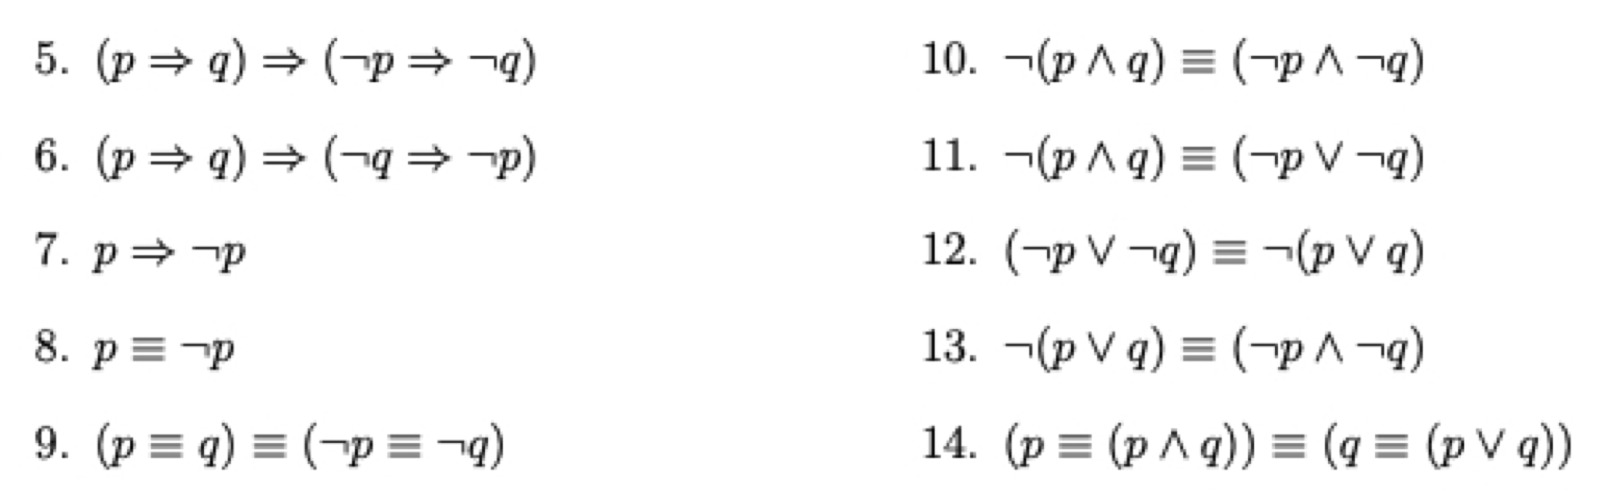
\includegraphics[width=0.6\textwidth]{images/esTableaux.jpeg}
            \label{fig:esTableaux1}
        \end{figure}
    \end{Exercise}
       
    
    
    \subsection{Tableaux LTL}
    \begin{Exercise}
    Svolgere i seguenti tableaux LTL:
        \begin{enumerate}
        \begin{minipage}{0.49\linewidth}
            \item \(p \land GF \neg p\)
            \item $\neg p \land X \neg p \land (q \cup p)$
            \item \(G p \land F \neg q\)
            \item \(G F p\)
        \end{minipage}
        \begin{minipage}{0.49\linewidth}
            \item \(p \lor G q\)
            \item \(G F(p \land X \neg p)\)
            \item \(G \neg p \land q U p\)
            \item $p \lor F(q \lor \neg p)$
        \end{minipage}
        \end{enumerate}
    \end{Exercise}
    
\end{document}